\chapter{HIỆN THỰC HỆ THỐNG}
\section{Phần cứng và sơ đồ nối dây}
\begin{figure}[H]\centering
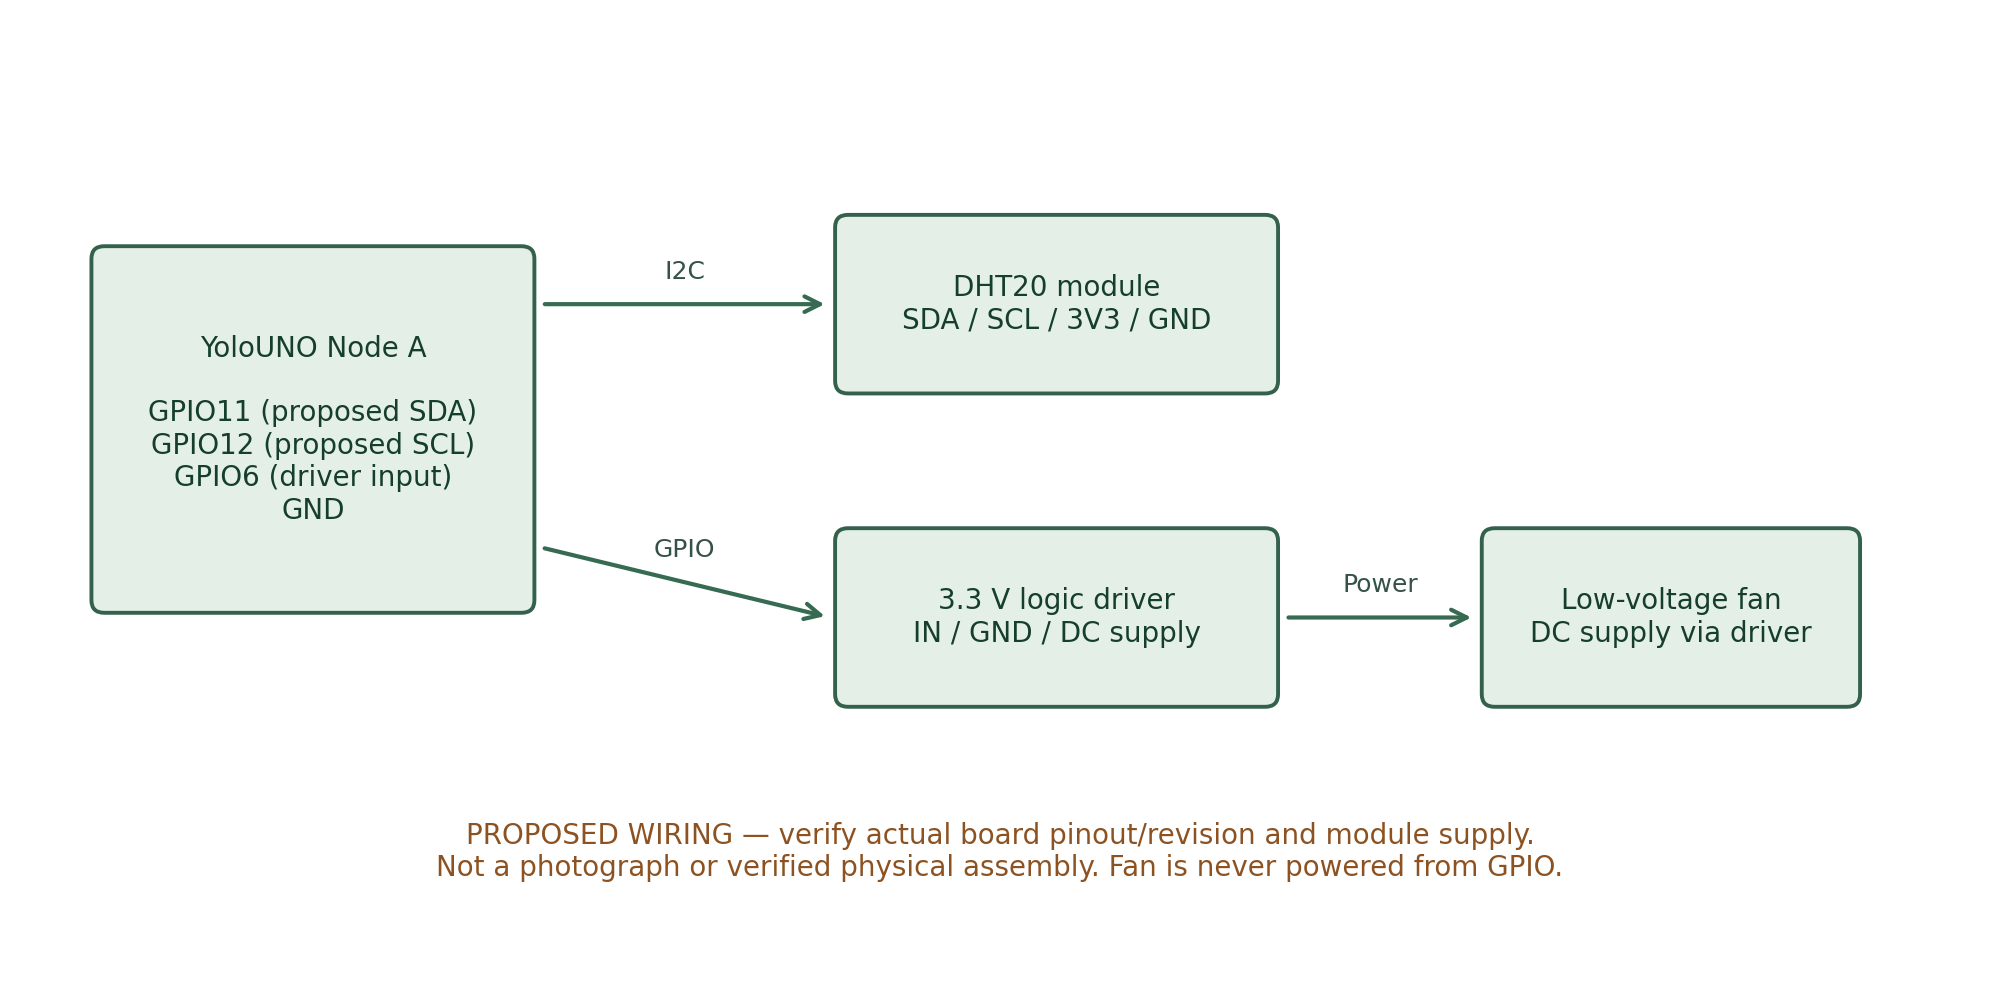
\includegraphics[width=\textwidth]{figures/wiring_proposed.png}
\caption{Sơ đồ nối dây đề xuất, chưa phải ảnh mạch đã lắp.}
\end{figure}
Chân đề xuất là GPIO11 cho SDA, GPIO12 cho SCL và GPIO6 cho tín hiệu driver. Các số này là GPIO thô của ESP32, không tự đồng nhất với nhãn D11/D12/D6 trên board. Trước khi nạp phải đối chiếu sơ đồ board thực tế, cổng I2C và thông số module. Đầu vào driver cần nhận mức logic 3,3~V; nguồn tải quạt cấp qua driver và mass tham chiếu theo module.

Board definition \code{firmware/boards/yolo_uno.json} là cấu hình build riêng của dự án: ESP32-S3, 240~MHz, flash 4~MB, DIO, không bật PSRAM và dùng variant generic với GPIO khai báo tường minh. Đây không phải khẳng định mọi phiên bản YoloUNO đều có cùng dung lượng flash. Mục đích là build trong cấu hình bộ nhớ bảo thủ; xác nhận revision và khả năng boot vẫn cần board thật.

\section{Firmware thiết bị}
\subsection{Node cảm biến/điều khiển và bridge (T06)}
Firmware dùng chung \code{main.cpp} với hai environment PlatformIO: \code{sensor} đặt \code{ROLE_SENSOR=1}, \code{bridge} đặt bằng 0. Ghim \code{espressif32@6.13.0}, Arduino-ESP32 2.0.17, ArduinoJson 6.21.5 và DHT20 0.3.2 để callback ESP-NOW và API không đổi ngoài dự kiến. Hai firmware đã build thành công; log ở \code{evidence/firmware_build.log}.

Sau boot, node đưa đầu ra quạt về tắt, tạo boot ID ngẫu nhiên, khởi tạo Wi-Fi/ESP-NOW, thêm peer với MAC và khóa cấu hình. Node sensor mở I2C, đọc DHT20 mỗi 2 giây. Chỉ khi mã trả về thành công mới đóng gói telemetry; khi lỗi, dừng phát mẫu đó và đưa đầu ra về tắt. Không thay một lần đọc lỗi bằng số 0 hoặc giá trị được sinh.

Bridge giải mã gói nhận và xuất Serial JSONL. Callback Wi-Fi chỉ kiểm tra MAC/độ dài/header rồi đẩy vào hàng đợi FreeRTOS tối đa 12 gói; JSON, Serial, ghi NVS và xử lý web nằm trong loop. Nếu hàng đợi đầy, gói có thể bị bỏ; sequence giúp nhận diện tình huống này trong phép đo thực.

Lệnh quạt dùng \emph{set trạng thái}, không dùng toggle. Node ghi command ID cuối vào NVS; ID lặp chỉ được ACK trạng thái đầu ra hiện tại, không áp dụng lại lệnh. Nếu bật quạt, lệnh có lease 30 giây rồi firmware tự đưa đầu ra về tắt. Telemetry tiếp theo công bố trạng thái mới. Khi lỗi cảm biến, đầu ra cũng tắt. Đây là chính sách của mô hình DC thí nghiệm, chưa phải chiến lược điều khiển thông gió hoàn chỉnh.

\subsection{Web server trên thiết bị (T07)}
Bridge chạy \code{WebServer} cổng 80, tạo AP \code{SmartRoom-Bridge}. Sau khi kết nối AP, trình duyệt mở \code{192.168.4.1}; trang tự viết lấy dữ liệu từ \code{/api/state}, hiển thị nhiệt độ, độ ẩm, fan và tuổi dữ liệu. API \code{/api/fan} nhận boolean và gửi \code{local_command} qua USB tới PC để dùng cùng cơ chế cấp ID/retry/ACK. Vì vậy điều khiển từ web bridge yêu cầu PC gateway đang chạy; trang vẫn xem được dữ liệu radio nếu PC ngừng.

Trang yêu cầu Basic Auth; mật khẩu AP, mật khẩu quản trị và khóa radio mẫu phải thay trong cấu hình local. Basic Auth trên HTTP không thay thế HTTPS; cấu hình này chỉ phục vụ mạng AP lab riêng. Hiện có bằng chứng build, chưa có screenshot web chạy trên board nên chưa nhận T07 hoàn tất.

\section{Truyền thông giữa các thiết bị}
\begin{table}[H]\centering\small
\caption{Khung ESP-NOW phiên bản 1, tổng cộng 25 byte}
\begin{tabular}{P{4cm}P{2.3cm}P{8cm}}
\toprule Trường & Số byte & Ý nghĩa \\ \midrule
magic, version, type & 2 + 1 + 1 & Nhận diện giao thức; telemetry/command/ACK. \\
boot, seq & 4 + 4 & Phiên khởi động và số thứ tự telemetry. \\
commandId & 4 & ID bền từ PC; đi qua bridge không thay đổi. \\
temperature, humidity & 4 + 4 & Số thực float hai đại lượng. \\
fan & 1 & Boolean mã hóa thành 0/1. \\
\bottomrule
\end{tabular}
\end{table}
Hai board cùng kiến trúc ESP32-S3 nên khung packed dùng định dạng little-endian hiện tại. Nếu bổ sung nền tảng khác cần serialization độc lập endian. Chống trùng tại PC dùng \code{(device,boot,seq)}; trong cùng boot, sequence không tăng sẽ bị bỏ. Boot ID ngẫu nhiên 32 bit có xác suất va chạm, và sequence 32 bit có thể wrap sau thời gian rất dài; phiên bản hiện tại chưa xử lý các trường hợp biên này thành giao thức tổng quát.

Ví dụ telemetry từ USB:
\begin{verbatim}
{"type":"telemetry","device":"room-node-01",
 "boot":1234,"seq":8,"temperature":27.6,
 "humidity":61.2,"fan":false}
\end{verbatim}
Gateway chấp nhận một dòng bị chia nhiều lần đọc Serial, bỏ log boot không phải JSON, từ chối object sai cấu trúc và giới hạn buffer. Giới hạn vật lý và tỷ lệ mất gói ESP-NOW chưa được đo. Bằng chứng cần bổ sung là log đồng thời ở hai board với cùng boot/seq và các phép đo khoảng cách, không phải ảnh build.

\section{IoT Gateway}
\subsection{Thu thập, lưu trữ và đường điều khiển (T08, T15)}
\code{gateway/core.py} chứa logic, \code{transports.py} chứa adapter Serial/mô phỏng/MQTT và \code{server.py} cung cấp HTTP. Khi nhận mẫu, gateway kiểm tra tên thiết bị, boot/seq kiểu integer, fan kiểu boolean, nhiệt độ hữu hạn trong $[-40,85]$ và độ ẩm trong $[0,100]$. Miền chấp nhận là hàng rào dữ liệu đầu vào, không phải sai số hay giới hạn đo đã thực nghiệm của cảm biến.

Bảng readings lưu mẫu; events lưu chuyển trạng thái; commands lưu yêu cầu điều khiển; outbox lưu topic/payload cần gửi. Ngưỡng và AI được tính trước khi lưu reading + event + outbox trong cùng giao dịch. Khi outbox đủ 100.000 bản tin, mẫu mới bị từ chối và báo lỗi thay vì âm thầm xóa dữ liệu chưa gửi. Đây là giới hạn theo số bản tin, chưa phải hạn mức tổng dung lượng đĩa.

Khi cloud nối lại, adapter đăng ký child bằng \code{v1/gateway/connect} trước khi flush telemetry. Topic, cấu trúc và tên child được triển khai theo Gateway API chuẩn \cite{gatewayapi}. Người dùng đã xác nhận Latest telemetry và nút RPC; gateway ghi các command có RPC ID và trạng thái applied với node mô phỏng. Bản tin telemetry có dạng:
\begin{verbatim}
Topic: v1/gateway/telemetry
{"room-node-01":[{"ts":1795000000000,"values":{
  "temperature":27.6,"humidity":61.2,"fan":false,
  "anomaly":false,"threshold_alarm":false,
  "data_source":"hardware"}}]}
\end{verbatim}
Timestamp là thời gian PC nhận, không phải thời điểm cảm biến lấy mẫu đã đồng bộ clock. Vì vậy không thể suy ra độ trễ radio hoặc end-to-end từ phép trừ timestamp không cùng hệ quy chiếu.

Outbox chỉ xóa sau khi Paho báo PUBACK QoS 1. Nếu broker đã nhận và PC tắt trước khi xóa, bản tin có thể gửi lại; hệ thống có ngữ nghĩa \emph{at least once}. PUBACK không xác nhận RuleChain hoặc widget đã cập nhật. Hiện readings/events chưa có chính sách lưu trữ cuốn chiếu nên cần theo dõi ổ đĩa khi chạy lâu.

RPC nhận từ cloud có dạng:
\begin{verbatim}
{"device":"room-node-01","data":{
  "id":14,"method":"setFan","params":true}}
\end{verbatim}
Gateway ghi pending và ánh xạ request ID cloud vào command ID local bền. Chỉ khi nhận ACK đúng ID/giá trị mới gửi:
\begin{verbatim}
Topic: v1/gateway/rpc
{"device":"room-node-01","id":14,
 "data":{"success":true,"fan":true,"detail":"Device ACK"}}
\end{verbatim}
\begin{figure}[H]\centering
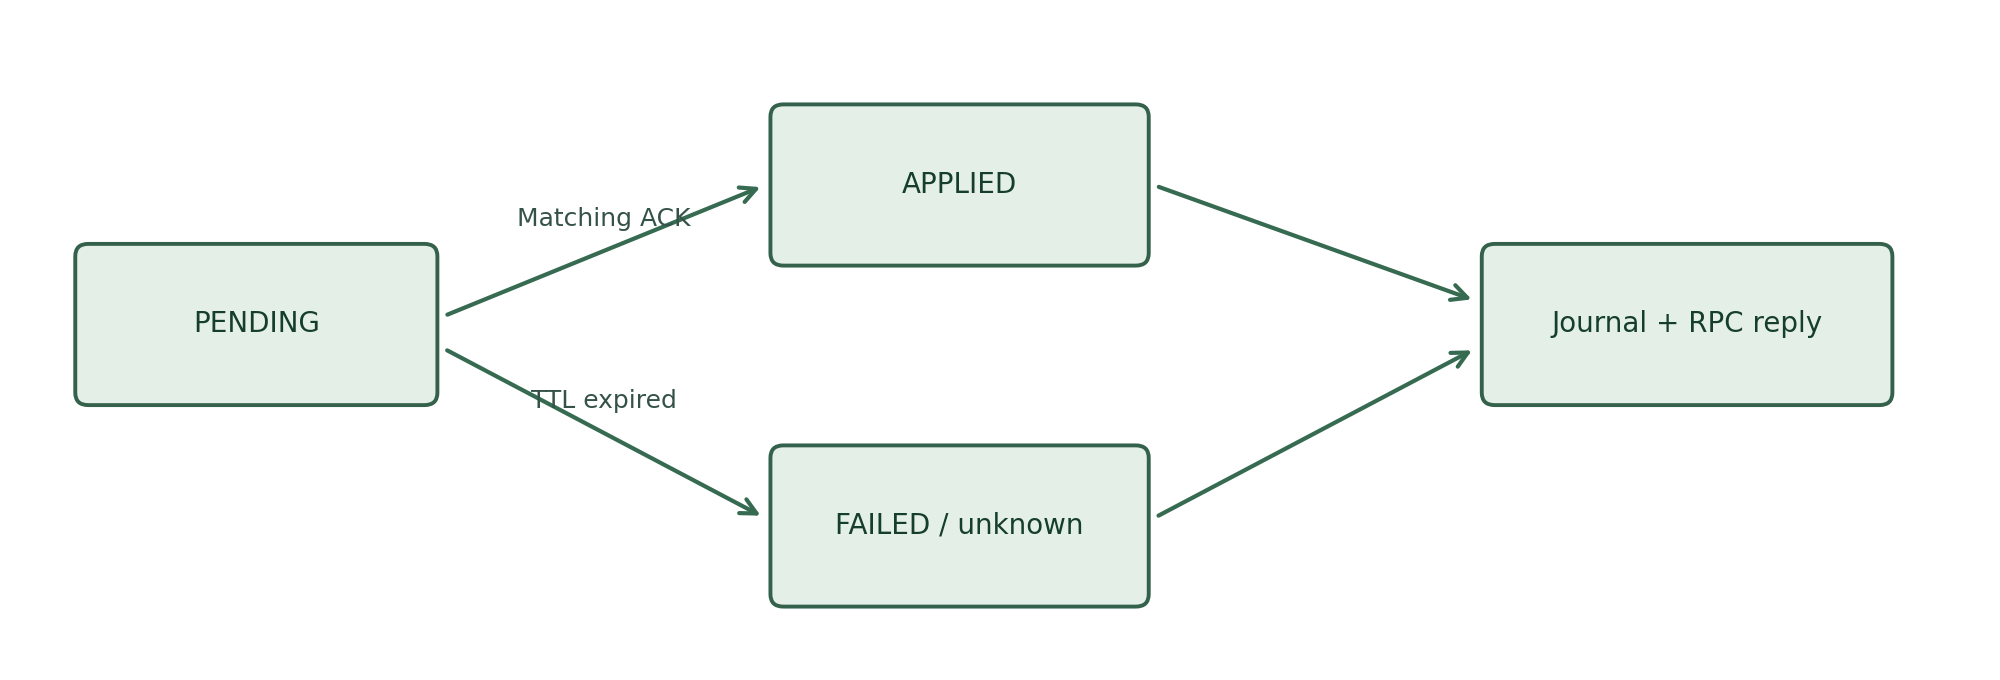
\includegraphics[width=\textwidth]{figures/command_state.png}
\caption{Lệnh hoàn thành bằng ACK; hết TTL không suy diễn trạng thái vật lý.}
\end{figure}
Mỗi thời điểm chỉ cho một lệnh pending để tránh retry bật/tắt đến đảo thứ tự. Trường hợp hết TTL được ghi failed; ACK đến muộn không đổi thành applied. Trạng thái thực tế vẫn theo telemetry, vì ACK có thể mất sau khi GPIO đã đổi. ACK xác nhận trạng thái đầu ra do firmware báo, chưa đo dòng điện hoặc tốc độ quạt.

Trong lần kiểm tra ngày 26/11, request ID RPC được dùng lại nhưng SQLite còn lệnh từ phiên cũ, khiến lệnh mới bị coi là lặp hoặc khác tham số. Bản sửa thêm phạm vi phiên MQTT vào khóa chống lặp; mỗi kết nối thành công có session ID riêng. ID lệnh local gửi xuống node vẫn tăng và lưu bền. Test kiểm tra cả lệnh cùng/khác giá trị giữa hai phiên và lệnh lặp trong cùng phiên. Sau khi khởi động lại bản sửa, người dùng xác nhận web--CoreIOT đồng bộ hai chiều; API gateway ghi các RPC ID 4, 5, 6 tương ứng lệnh 18, 19, 20 đều applied. Minh chứng nằm ở \code{evidence/fan_sync_live_check.json}; sensor vẫn mô phỏng.

\subsection{Giao diện giám sát và điều khiển (T10)}
HTTP server mặc định chỉ bind \code{127.0.0.1}. API \code{/api/state} trả reading mới nhất, 120 mẫu gần nhất, 60 sự kiện gần nhất, 20 lệnh gần nhất và số outbox. Sau 15 giây không có mẫu mới, trạng thái hiển thị stale. Dashboard dùng một switch bật/tắt và phân biệt pending/applied/failed. Switch cập nhật từ telemetry hoặc ACK mới hơn bản tin gần nhất, tạm khóa khi chờ xác nhận hoặc mất dữ liệu mới. Cập nhật do RPC không tự phát thêm POST từ web, tránh vòng lặp điều khiển. Phản hồi HTTP 202 chỉ có nghĩa nhận yêu cầu, không phải lệnh đã thực thi.

\begin{figure}[H]\centering
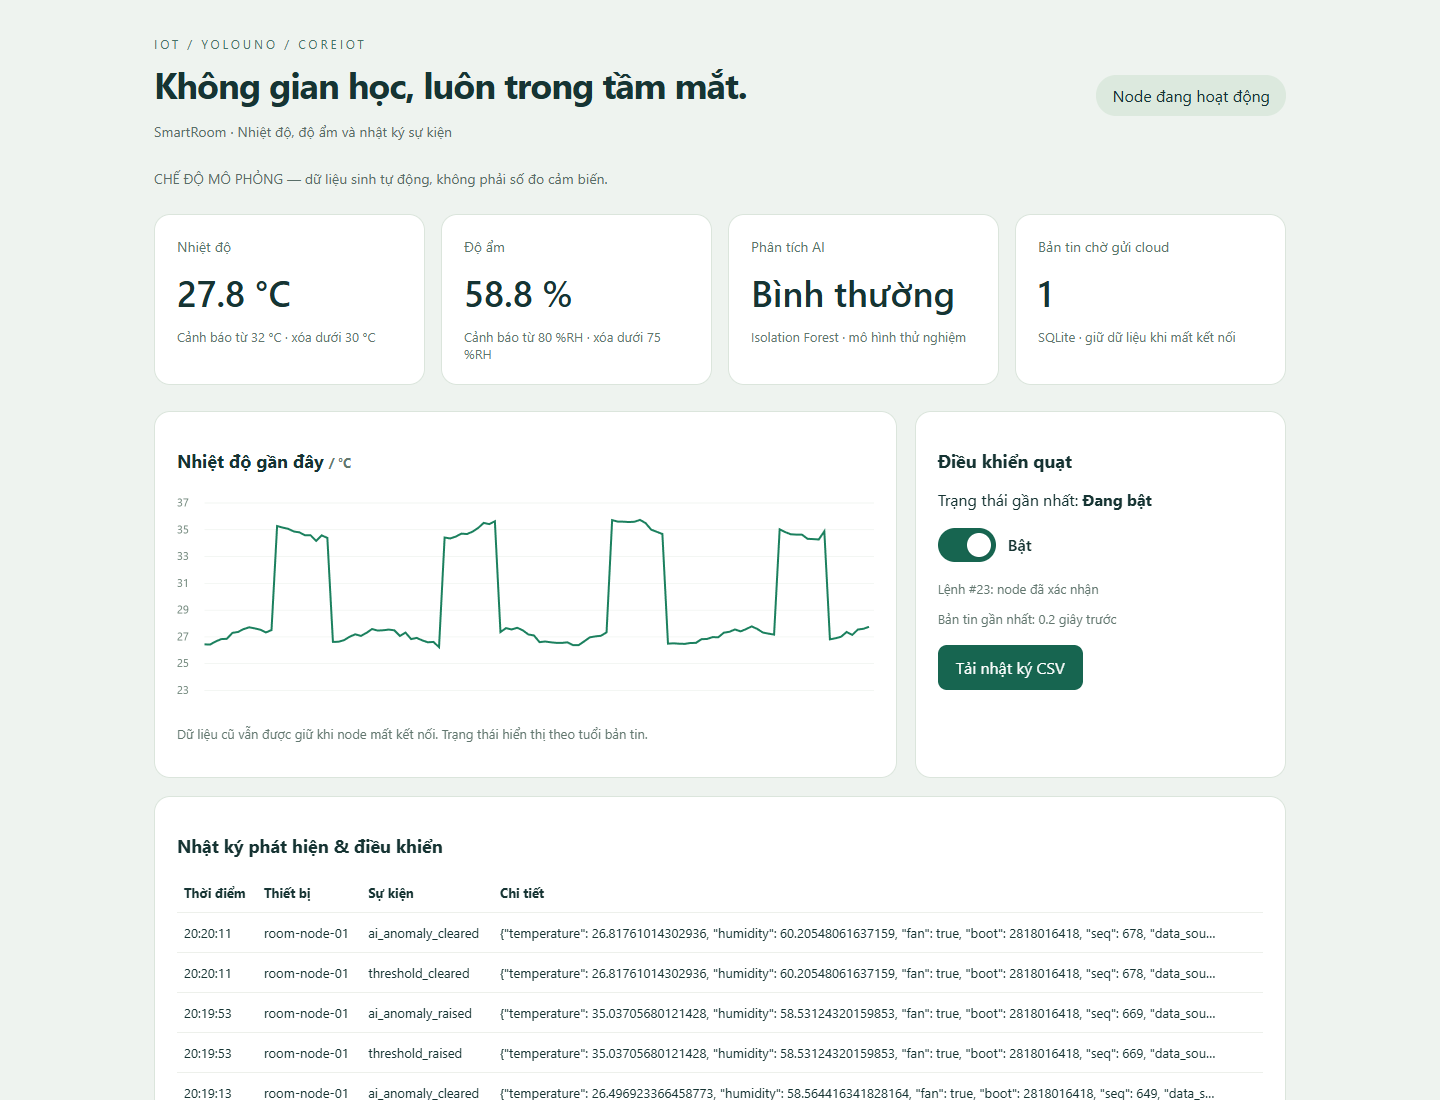
\includegraphics[width=\textwidth,height=.70\textheight,keepaspectratio]{../evidence/dashboard_current_desktop.png}
\caption{Ảnh Chrome ngày 26/11 của gateway đang chạy tại cổng 8081: switch quạt và AI đã nạp model; nguồn sensor mô phỏng. Chụp chỉ đọc, không gửi lệnh trong lượt chụp.}
\end{figure}
Nhật ký được ghi SQLite và xuất CSV toàn bộ events qua \code{/api/events.csv}. Hiển thị bảng dùng \code{textContent} để dữ liệu không bị thực thi như HTML. API điều khiển kiểm tra Origin cùng Host khi trình duyệt cung cấp; mặc định loopback hạn chế truy cập mạng ngoài. Phiên bản hiện tại chưa có tài khoản người dùng, reverse proxy HTTPS hoặc phân quyền nhiều người, nên không mở trực tiếp cổng này ra Internet.

\section{Trí tuệ nhân tạo trên gateway (T09)}
\subsection{Thu thập và chuẩn bị dữ liệu}
\code{ai/train.py} có hai chế độ. Chế độ mặc định sinh 1.500 mẫu bình thường để train; tập test độc lập gồm 800 bình thường, 200 nóng và 200 ẩm cao, tổng 1.200. Bộ sinh dùng seed 2353007. Mẫu bình thường có phân bố quanh 27~°C và 60~\%RH; các tình huống nóng/ẩm được đặt phân bố khác để kiểm tra pipeline. Vì những tình huống này tách khá rõ, accuracy cao không phải bằng chứng về độ khó thực tế.

Chế độ CSV yêu cầu cột \code{temperature,humidity,label}, nhãn 0/1 và thứ tự thời gian. 60\% đầu là miền train, chỉ lấy mẫu normal trong phần này; 40\% cuối dành cho test. Cần ít nhất 100 mẫu normal train và 50 mẫu test hữu hạn có đủ hai lớp. Khi thu thập thực tế, phải ghi bối cảnh, phiên/phòng và cách gán nhãn; không tự tạo nhãn bằng đúng luật ngưỡng rồi dùng kết quả để khẳng định AI vượt luật đó.

Bản cập nhật kiểm tra toàn bộ CSV trước khi chia tập: đủ cột; nhãn đúng 0 hoặc 1, không làm tròn nhãn thập phân; nhiệt độ hữu hạn trong $[-40,85]$ và độ ẩm trong $[0,100]$. Miền này khớp hàng rào dữ liệu gateway, không phải chứng nhận cảm biến. Thứ tự thời gian vẫn do người cung cấp CSV đảm bảo vì định dạng hiện không bắt buộc cột timestamp.

\subsection{Huấn luyện và đánh giá}
Isolation Forest gồm 100 cây, contamination 0,02, random state cố định và chạy CPU một job. Không có bước chọn hyperparameter dựa trên tập test. Mô hình trả decision score; giá trị âm được đánh dấu anomaly. Tài liệu thư viện mô tả tham số và quy ước score này \cite{isolation}.

Các chỉ số tính trên tập test độc lập là precision, recall, F1 và accuracy. Với lớp bất thường, đặt TP là phát hiện đúng, FP là báo động giả, FN là bỏ sót:
\[
P=\frac{TP}{TP+FP},\qquad R=\frac{TP}{TP+FN},\qquad
F_1=\frac{2PR}{P+R}.
\]
Số liệu cụ thể và confusion matrix nằm ở Chương 4; file CSV lưu từng dự đoán để tái kiểm tra. Tách đánh giá AI khỏi đánh giá ngưỡng tránh đồng nhất hai cơ chế.

Module \code{ai/evaluate.py} nạp model cố định, kiểm tra SHA-256 và so sánh với luật ngưỡng nhiệt độ $\geq32$ hoặc độ ẩm $\geq80$. Luật so sánh từng mẫu không có hysteresis; hysteresis của ứng dụng đã được kiểm tra bằng chuỗi riêng. Đánh giá gồm bộ gốc, năm seed mới cùng phân bố, trường hợp normal dịch phân bố, lạnh chưa có trong tập huấn luyện và bất thường hiếm. Không huấn luyện lại, tìm ngưỡng hoặc đổi contamination sau khi xem kết quả. Nhãn do kịch bản sinh dữ liệu quy định, không phải số đo thực. Decision score không phải xác suất tin cậy; không đổi score thành phần trăm chính xác.

\subsection{Triển khai mô hình}
Model được xuất \code{ai/model.joblib} và nạp một lần khi gateway khởi động. Mỗi mẫu hợp lệ được bổ sung \code{anomaly_score}, \code{anomaly}, \code{inference_ms} và \code{ai_available}. Nếu chưa có model, giao diện hiển thị chưa có model; không gán nhãn ``bình thường'' giả. Model đặt trên PC, không đưa lên ESP32 nên không đăng ký TinyML.

Khi thay dữ liệu hoặc phiên bản scikit-learn, nên train lại và khởi động lại gateway. Chỉ nạp model do nhóm tự tạo hoặc từ nguồn tin cậy. Bản model sinh phục vụ demo có thể khác rõ dữ liệu phòng học thật, vì vậy cần một giai đoạn thu dữ liệu trước khi dùng score làm cơ sở vận hành.

\section{Nền tảng CoreIOT}
\subsection{Device Profile, template và dashboard (T11)}
Nhóm sử dụng cổng web \url{https://app.coreiot.io/home}. Các ảnh và cấu hình thực đã được lưu trong \code{evidence/coreiot/}. Export \code{smartroom_co3037.json} có bốn widget: Temperature, Humidity, bảng Alarms và Single Switch Fan. Alias cảm biến tìm \code{room-node-01}; switch chọn cùng hệ thống thiết bị và lấy time-series \code{fan}. API local trước đó ghi nguồn \code{simulation}, RPC ID applied và outbox bằng 0. MQTT dùng \code{app.coreiot.io:1883} theo tài liệu CoreIOT \cite{coreiotconnect}.

\begin{figure}[H]\centering
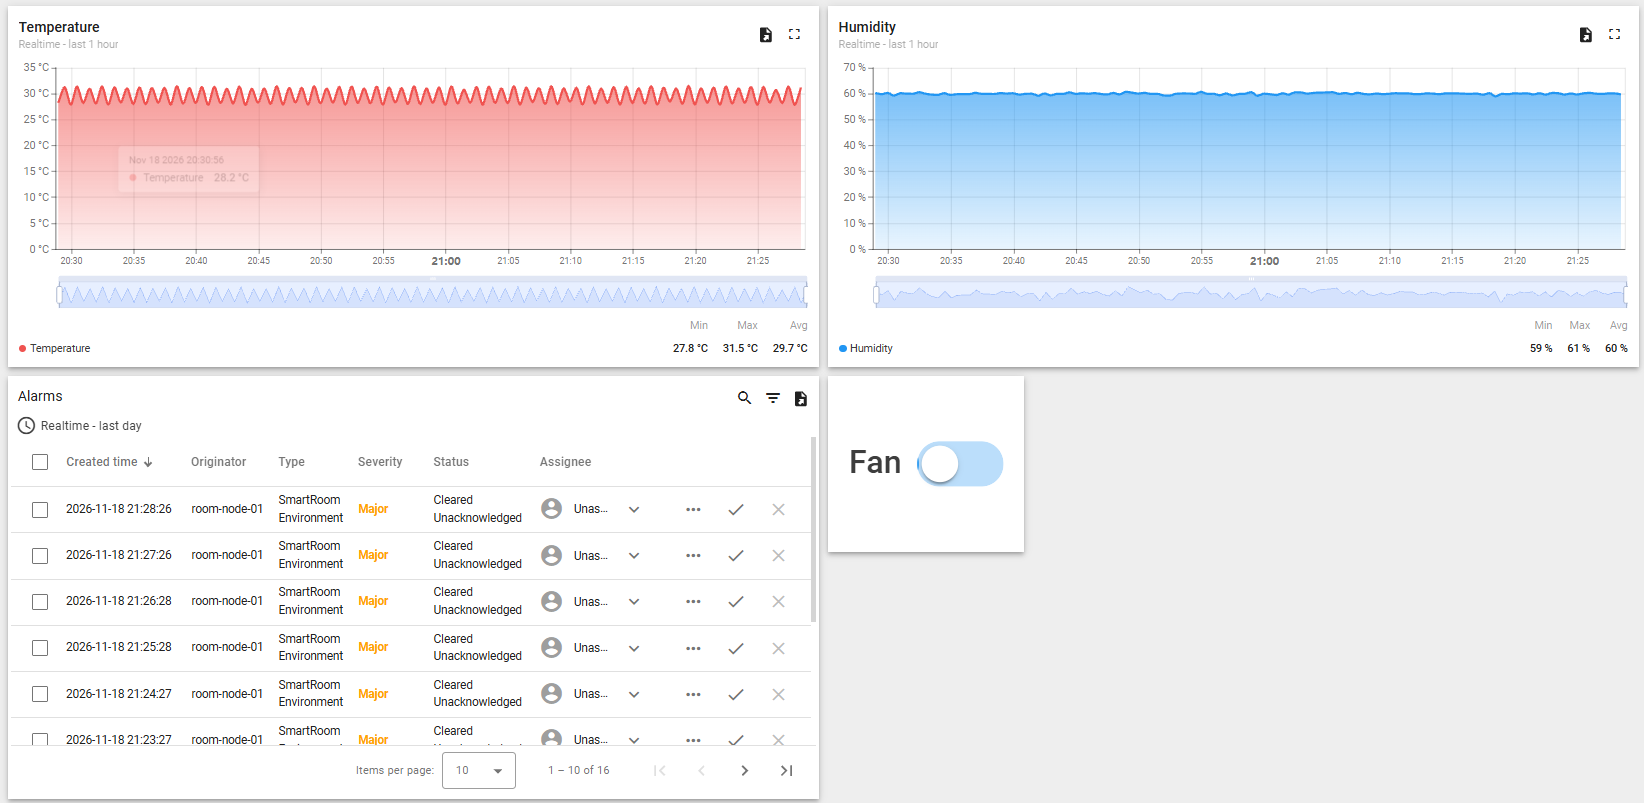
\includegraphics[width=\textwidth,height=.58\textheight,keepaspectratio]{../evidence/coreiot/SmartRoom_Dashboard.png}
\caption{Ảnh CoreIOT gốc lưu ngày 18/11: hai biểu đồ, Single Switch Fan và alarm; chưa có các thẻ AI bổ sung ngày 26/11. Nguồn cảm biến mô phỏng.}
\label{fig:coreiot-dashboard}
\end{figure}

\code{coreiot/smartroom_dashboard.json} giữ hai time-series widget và alarm table từ template Thermostats chính thức. File nguồn, commit SHA, SHA-256 và giấy phép Apache-2.0 được lưu trong \code{coreiot/templates/}. Dự án thay alias thành \code{room-node-01}, bố cục và nhãn; bỏ map và form quản trị không phục vụ đề tài. Phần giao diện widget kế thừa không được trình bày như mã hoàn toàn do nhóm viết.

Ảnh và export gốc xác nhận trục Humidity dùng đơn vị \%. Bản ngày 18/11 còn AVG mỗi 30 giây; bản mới \code{smartroom_dashboard_20261126.json} đã xác nhận cả hai biểu đồ dùng aggregation NONE, cửa sổ riêng 1 giờ. Các đỉnh ngắn được hiển thị bằng dữ liệu gốc; RuleChain vẫn xét telemetry đầu vào. Hai bản export được giữ riêng theo ngày, không sửa cấu hình cũ để giả như thay đổi đã có trước đó.

Bản \code{coreiot/smartroom_dashboard_rpc.json} trước đây được dùng khởi tạo hai RPC Button đặt method \code{setFan}, params boolean true/false và target alias sensor. Lệnh dùng two-way, timeout 10 giây; người dùng đã xác nhận vận hành và gateway ghi trạng thái applied cho các RPC ID. File này được giữ làm cấu hình ban đầu và fixture kiểm thử, không yêu cầu import lại khi đã có dashboard đang dùng.

Export xác nhận widget \code{system.single_switch} có Initial state=GET\_TIME\_SERIES, key \code{fan}; On/Off đều EXECUTE\_RPC, method \code{setFan}, tham số boolean true/false. Không có lời gọi getFan ở bước lấy trạng thái. Người dùng xác nhận RPC chạy và API local có command applied; chưa dùng ảnh động tác gạt thay cho phản hồi node. Người dùng sửa thủ công nên công cụ REST/DPAPI chỉ là tùy chọn. Dashboard export không chứa runtime ID; URL đang dùng cần đối chiếu riêng, không suy ra từ tiêu đề.

\subsubsection{Các thẻ AI bổ sung ngày 26/11/2026}
Sau khi đánh giá AI và sửa đồng bộ switch, nhóm bổ sung các thẻ quan sát trực tiếp kết quả phân tích trên CoreIOT. Người dùng cung cấp ảnh và xác nhận hoàn tất cấu hình trong trao đổi. Tất cả đọc child \code{room-node-01}; Status widget lấy trạng thái bằng \emph{Get time series}, không gọi RPC để lấy trạng thái model. Các tiêu đề dùng tiếng Anh để thống nhất giao diện.

\begin{longtable}{P{3.3cm}P{3.6cm}P{7cm}}
\caption{Các thẻ trên dashboard sau khi bổ sung AI}\label{tab:coreiot-ai-cards}\\
\toprule Tiêu đề & Widget / key & Ý nghĩa hiển thị \\ \midrule
AI Availability & Status widget; \code{ai_available} & True: MODEL READY; false: MODEL UNAVAILABLE. Xác nhận model đã nạp, không phải độ chính xác của AI. \\
Anomaly Score & Value card; \code{anomaly_score} & Score 4 chữ số thập phân, không có đơn vị; giá trị âm được model đánh dấu bất thường. \\
Anomaly Detection & Status widget; \code{anomaly} & Cờ true: ANOMALY, nền đỏ; false: NORMAL, nền xanh. Export dùng điều kiện On khi kết quả bằng false. \\
Inference Time & Value card; \code{inference_ms} & Thời gian suy luận trên PC, đơn vị ms; không phải độ trễ sensor--cloud. \\
Data Source & Value card; \code{data_source} & Hiện simulation để nhận biết dữ liệu sinh; hardware chỉ khi thật sự chạy từ bridge. \\
Fan & Single Switch; \code{fan} & Đọc trạng thái fan và gửi \code{setFan} boolean; đồng bộ hai chiều đã kiểm tra với node mô phỏng. \\
\bottomrule
\end{longtable}

Ảnh mới đã lưu hiển thị MODEL READY, score 0,2435, NORMAL, inference 6~ms và nguồn simulation; score không âm khớp với trạng thái NORMAL. Hai biểu đồ hiển thị nhiệt độ khoảng 26,1--35,9~°C và độ ẩm 56--64\% trong cửa sổ đang xem; bảng Alarms có các bản ghi SmartRoom Environment đã clear. Biểu tượng score đã đổi từ tam giác cảnh báo đỏ cố định sang biểu tượng thông tin xanh để tránh làm người xem hiểu nhầm mọi score đều là cảnh báo. Đây là một quan sát giao diện, không phải benchmark hoặc phép đo lặp. Người dùng xác nhận đã sửa On/Off; ảnh lưu trực tiếp thể hiện trạng thái normal, chưa là minh chứng riêng cho mọi lần chuyển trạng thái.

Nội dung quan sát, kích thước và SHA-256 ảnh/export mới được ghi tại \code{evidence/coreiot/dashboard_ai_user_check.json}. Hình \ref{fig:coreiot-dashboard} giữ ảnh gốc ngày 18/11; ảnh và JSON ngày 26/11 được lưu riêng. Export mới có 9 widget: 2 biểu đồ, bảng Alarms, Fan, 3 Value card và 2 Status widget. Kiểm tra tĩnh đạt 15/15 điều kiện, gồm layout hợp lệ, hai biểu đồ NONE, các key AI và RPC boolean; kết quả ở \code{evidence/coreiot_dashboard_ai_check.json}.

Riêng Anomaly Detection, \code{compareToValue=false} làm cờ anomaly=false chọn bộ On với chữ Normal/nền xanh; anomaly=true chọn bộ Off với chữ Anomaly/nền đỏ. Đây là ánh xạ hợp lệ đã được đối chiếu trên JSON, không đổi ý nghĩa cờ AI. AI Availability dùng \code{compareToValue=true}, On là Model ready và Off là Model Unavailable. Ba Value card có type latest, lần lượt đọc score, inference và nguồn dữ liệu; score dùng 4 chữ số thập phân, inference có đơn vị ms và 2 chữ số. Giá trị trên thẻ là telemetry gần nhất: khi đánh giá hoạt động cần kiểm tra thời gian cập nhật, không chỉ nhìn chữ MODEL READY.

\IfFileExists{../evidence/coreiot/SmartRoom_Dashboard_20261126.png}{%
\begin{figure}[H]\centering
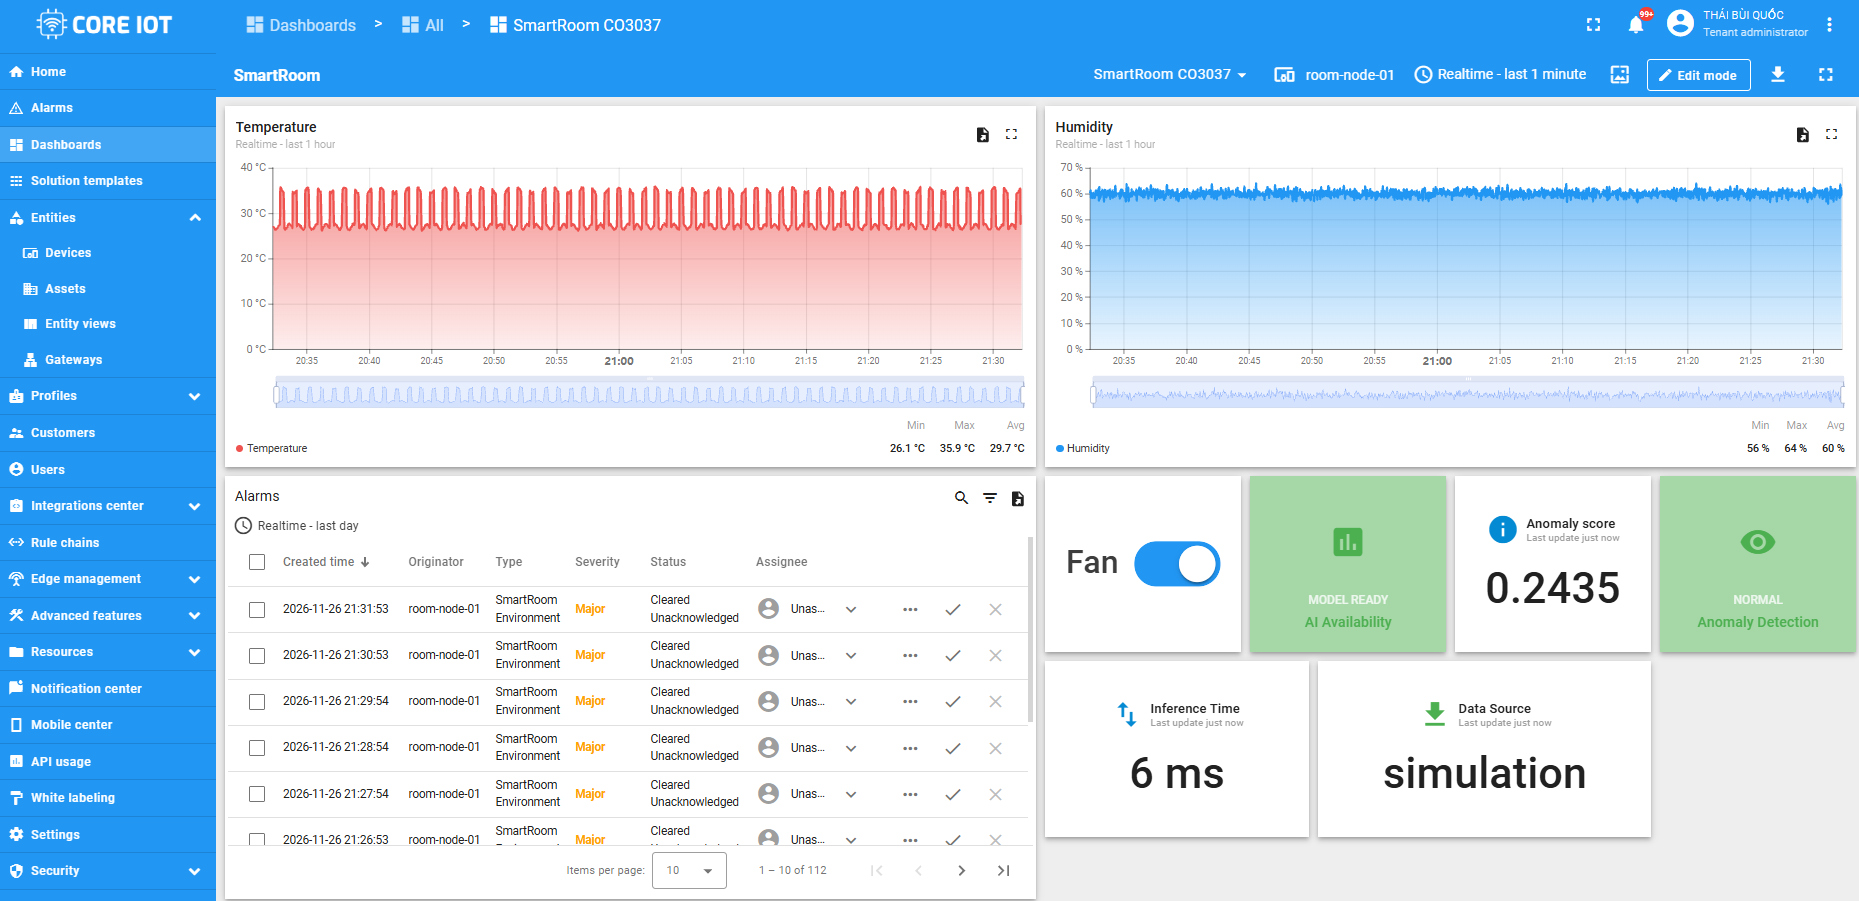
\includegraphics[width=\textwidth,height=.68\textheight,keepaspectratio]{../evidence/coreiot/SmartRoom_Dashboard_20261126.png}
\caption{Dashboard CoreIOT bổ sung các thẻ AI; ảnh người dùng lưu ngày 26/11, nguồn dữ liệu mô phỏng.}
\label{fig:coreiot-dashboard-updated}
\end{figure}
}{%
Ảnh mới đã được xem trong trao đổi nhưng chưa có file gốc tại đường dẫn minh chứng khi dựng PDF. Nhóm cần lưu \code{evidence/coreiot/SmartRoom_Dashboard_20261126.png} để ảnh được tự động nhúng ở lần dựng tiếp theo; bảng cấu hình và quan sát ở trên được giữ rõ nguồn.
}

\subsection{RuleChain và notification (T12, T13)}
RuleChain mới tên \code{SmartRoom alarms}, không đặt làm root toàn tài khoản. Nhánh Post telemetry được lưu timeseries rồi lọc điều kiện nhiệt độ $\geq32$~°C hoặc độ ẩm $\geq80$~\%RH hoặc anomaly=true. Nhánh True tạo alarm type \code{SmartRoom Environment}, mức MAJOR. Nhánh False kiểm tra điều kiện phục hồi: nhiệt độ $\leq30$, độ ẩm $\leq75$ và không anomaly; chỉ khi đạt mới clear. Vùng giữa giữ alarm hiện tại.

Export \code{root_rule_chain.json} xác nhận Post telemetry đi qua bộ lọc \code{metadata.deviceName === "room-node-01"}; True gọi SmartRoom alarms, False lưu timeseries cho các thiết bị khác. Nhánh RPC Request to Device vẫn tới RPC Call Request. Không còn đường lưu telemetry trực tiếp trùng lặp cho SmartRoom ở Root.

\begin{figure}[H]\centering
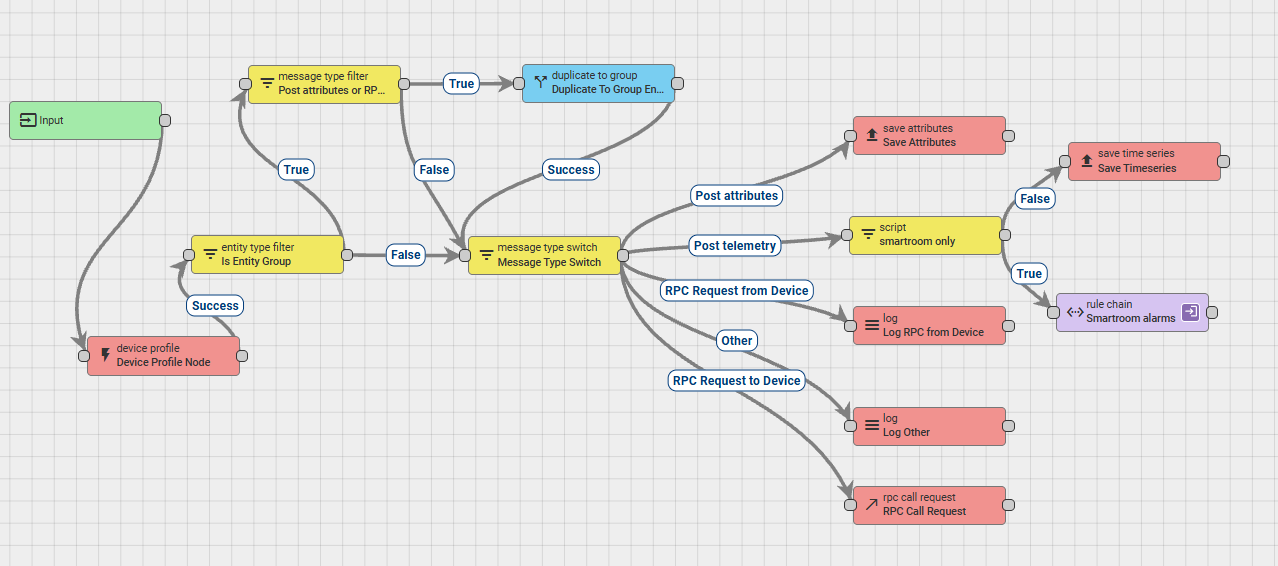
\includegraphics[width=\textwidth,height=.36\textheight,keepaspectratio]{../evidence/coreiot/Rule_chains_root.png}
\caption{Root Rule Chain đã cấu hình trên tài khoản: lọc riêng SmartRoom và giữ đường RPC.}
\label{fig:coreiot-root}
\end{figure}

Export \code{smartroom_alarms.json} xác nhận chuỗi Telemetry only $\rightarrow$ Save timeseries $\rightarrow$ High or anomaly; nhánh True tạo alarm, nhánh False kiểm tra điều kiện phục hồi trước khi clear. Hai action dùng cùng alarm type \code{SmartRoom Environment}; severity tạo là MAJOR.

\begin{figure}[H]\centering
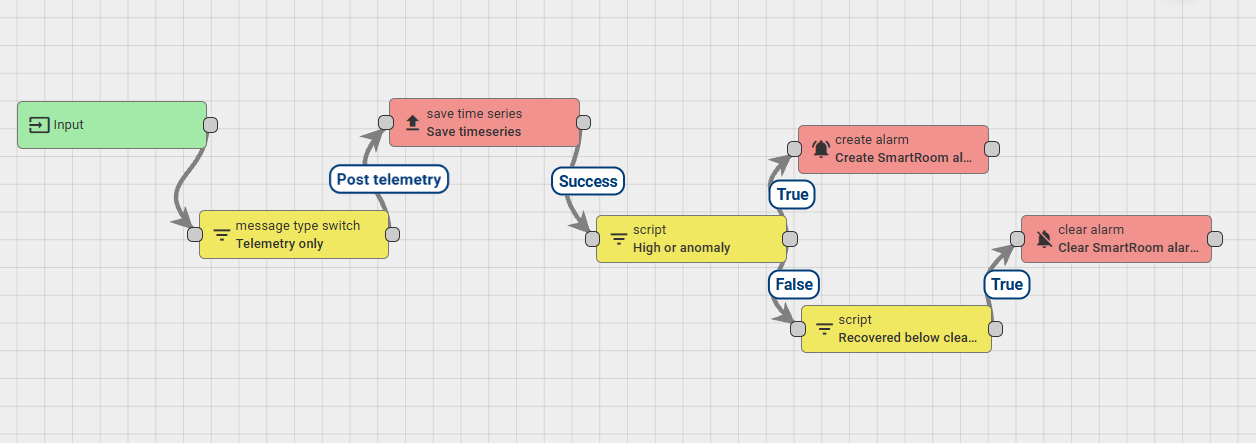
\includegraphics[width=\textwidth,height=.34\textheight,keepaspectratio]{../evidence/coreiot/Rule_chains_SmartRoom_alarms.png}
\caption{SmartRoom alarms thực: tạo alarm và clear với điều kiện phục hồi có hysteresis.}
\label{fig:coreiot-alarms}
\end{figure}

Ảnh dashboard ghi các alarm Major của \code{room-node-01} đã chuyển Cleared Unacknowledged. Ảnh Notification hiển thị cả New alarm và Alarm cleared qua nhiều đợt dữ liệu mô phỏng, xác nhận tạo, phục hồi và gửi Web notification.

\begin{figure}[H]\centering
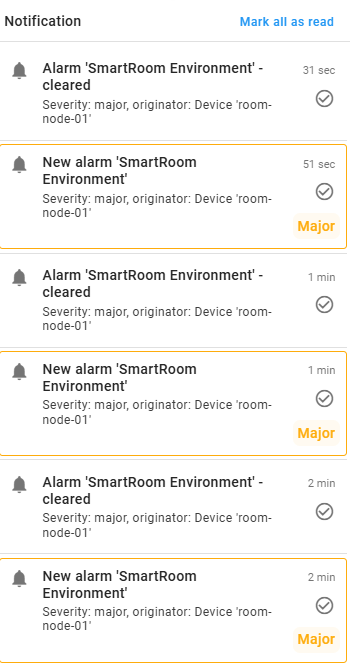
\includegraphics[width=.48\textwidth,height=.63\textheight,keepaspectratio]{../evidence/coreiot/Notification.png}
\caption{Thông báo Web đã nhận cho cả tạo và clear SmartRoom Environment trên CoreIOT.}
\label{fig:coreiot-notifications}
\end{figure}

Thông báo đã có trên tài khoản nên không tạo thêm rule trùng lặp. Chưa có export recipient/template/notification rule nên không khẳng định nhóm tự viết các cấu hình đó. Chưa kiểm chứng email/SMTP. Ảnh gốc và ba JSON export được giữ nguyên; SHA-256 và kết quả kiểm tra nằm ở \code{evidence/coreiot_export_check.json}. Không suy ra độ trễ định lượng từ nhãn thời gian tương đối trên ảnh.

\subsection{Cập nhật OTA (T14)}
Không triển khai. Dự án nạp firmware qua USB bằng PlatformIO; không có phép đo thời gian OTA hoặc phiên bản trước/sau để nhận điểm T14.

\section{Tính năng nâng cao (N06)}
Dashboard riêng không chỉ hiển thị: nó phát hiện chuyển trạng thái threshold/AI, lưu journal bền với thiết bị và timestamp, cho xem lịch sử, xuất CSV và theo dõi lệnh. Sự kiện chỉ ghi khi trạng thái đổi; nhiệt độ lắc quanh 31~°C sau alarm 32~°C không sinh chuỗi cảnh báo/xóa liên tục. Các hành vi này được kiểm thử tự động và quay/chụp trên trình duyệt với node mô phỏng.

N01--N05 và N07 không triển khai. Việc dùng AI để trợ giúp viết code không có nghĩa sản phẩm chứa trợ lý LLM N01. Giao diện responsive được kiểm tra ở chiều rộng 390 px nhưng không gọi là ứng dụng mobile N05.
